\documentclass{beamer}
\usepackage{hyperref}
\usepackage[T1]{fontenc}
\usepackage{ctex}
\usepackage[english]{babel}

\UseRawInputEncoding

% Cannot enable in Xelatex
\usepackage{pgfpages}
% \setbeameroption{hide notes} % Only slides
% \setbeameroption{show only notes} % Only notes
% \setbeameroption{show notes on second screen}

% other packages
\usepackage{latexsym,amsmath,xcolor,multicol,booktabs,calligra}
\usepackage{graphicx,listings,stackengine}
\usepackage{animate}

\definecolor{best}{rgb}{.8, .96, .94}
\usepackage{xcolor, colortbl}

% *************************** Additional package *****************************
\usepackage[linesnumbered,ruled,vlined]{algorithm2e}
\SetKwComment{Comment}{/* }{ */}   % The argument will be surrounded by /* ... */
\SetAlCapFnt{\footnotesize}        % Make caption text smaller
\SetAlCapNameFnt{\footnotesize}    % Make "Algorithm" label smaller

% \usepackage{algorithmic}
\usepackage{comment}
\usepackage{multicol}
\usepackage{multirow}
% \usepackage{subfigure}
\usepackage{subcaption}
\usepackage{verbatim}
\usepackage[font=scriptsize]{caption}   % Caption in Figures and Tables

%% Enable only in Xelatex
% \usepackage{pstricks}

% Set hyperlink colors
\begin{comment}
\hypersetup{
    colorlinks=true,
    linkcolor=darkblue,  % Color para enlaces internos
    filecolor=darkblue,  % Color para enlaces a archivos
    urlcolor=darkblue    % Color para URLs
}
\end{comment}

\author[IA-PUCP]{Artificial Intelligence Summer Camp - 2025}

\title{Introducción a Network Analytics}
% \subtitle{Presentation}
\institute [Artificial Intelligence Summer Camp - 2025] 
{
\vspace*{-0.1cm}
% \includegraphics[width=1.6cm]{pic/pucp.png}
\hspace*{0.25cm}~%

\includegraphics[width=2.0cm]{pic/iapucp_logo.jpg}
\hspace*{0.25cm}~%
% \includegraphics[width=1.4cm]{pic/unmsm.png}
\vspace*{0.35cm}\\

Inteligencia Artificial PUCP (IA-PUCP)}

\date{\scriptsize January 14, 2025}
\usepackage{YTU}

% defs
\def\cmd#1{\texttt{\color{red}\footnotesize $\backslash$#1}}
\def\env#1{\texttt{\color{blue}\footnotesize #1}}
\definecolor{deepblue}{rgb}{0,0,0.5}
\definecolor{deepred}{rgb}{0.6,0,0}
\definecolor{deepgreen}{rgb}{0,0.5,0}
\definecolor{halfgray}{gray}{0.55}

\lstset{
    basicstyle=\ttfamily\small,
    keywordstyle=\bfseries\color{deepblue},
    emphstyle=\ttfamily\color{deepred},    % Custom highlighting style
    stringstyle=\color{deepgreen},
    numbers=left,
    numberstyle=\small\color{halfgray},
    rulesepcolor=\color{red!20!green!20!blue!20},
    frame=shadowbox,
}

\begin{document}

\begin{frame}
    \titlepage
    \begin{figure}[ht!]
        \begin{center}
            % 
\includegraphics[width=0.2\linewidth]{pic/YTU_logo.jpg}
       \end{center}
    \end{figure}
    
    \begin{note}
        {Introduce your self}
    \end{note}
\end{frame}

\begin{frame}
    \tableofcontents[sectionstyle=show,subsectionstyle=show/shaded/hide,subsubsectionstyle=show/shaded/hide]
    % \tableofcontents[sectionstyle=show,subsectionstyle=hide,subsubsectionstyle=hide]
\end{frame}

\section{Section one}
    \begin{frame}{Basic}
        Graph is a data structure and is defined by $G = (V, E)$, where $V$ is the set of nodes and $E$ is the set of edges.
        
        \begin{figure}[ht!]
            \centering
            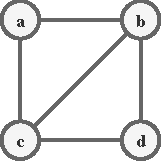
\includegraphics[width=0.25\linewidth]{pic/graph_example.pdf}
            \caption{Graph example.}
            \label{fig:graph}
        \end{figure}

        \begin{note}
            {Introduce your self}
        \end{note}
    \end{frame}
    
    \begin{frame}{Two columns}
        \begin{columns}[t] % The "c" option specifies centered vertical alignment while the "t" option is used for top vertical alignment
            \begin{column}{0.5\textwidth}
                \begin{itemize}
                    \item Homogeneous graph
                    \item Heterogeneous graph
                    \item Directed graph
                    \item Undirected graph
                    \item Weighted graph
                    \item Bipartite graph
                    \item Complete graph
                    \item Degree
                    \item Density
                    \item Diameter
                \end{itemize}
            \end{column}
            
            \begin{column}{0.5\textwidth}
                \begin{figure}[ht!]
                    \centering
                    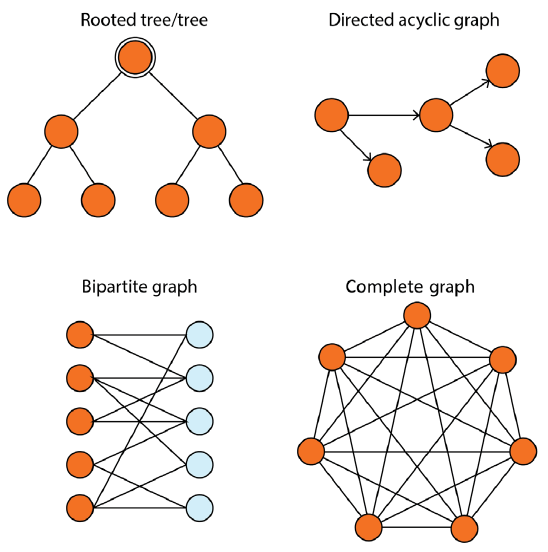
\includegraphics[width=1.0\linewidth]{pic/common_type_graph.png}
                    \caption{Common type of graphs. Adapted from \cite{labonne2023hands}.}
                    % \caption*{Adapted from \cite{labonne2023hands}.}
                    \label{fig:graph_types}
                \end{figure}
            \end{column}
        \end{columns}
        
        \begin{note}
            {Write your notes here}
        \end{note}
    \end{frame}

    \begin{frame}{Items multicolumns}
        \begin{multicols}{2}
            \begin{itemize}
                \item Computer vision
                \item Natural language processing
                \item Recommender systems
                \item Program analysis
                \item Knowledge graphs
                \item Bioinformatics
                \item Chemistry
                \item Biology
                \item Physic
                \item Anomaly detection
                \item Urban intelligence
                \item Financial transaction
                \item ...
            \end{itemize}
        \end{multicols}

        \begin{note}
            {Write your notes here}
        \end{note}
    \end{frame}

    \begin{frame}{Items and subitems}
        \begin{columns}[t] % The "c" option specifies centered vertical alignment while the "t" option is used for top vertical alignment
            \begin{column}{0.5\textwidth}
                \begin{enumerate}
                    \item Class 1
                    \item Class 2
                    \item Class 3
                    \begin{itemize}
                        \item[n+e] Student 1
                    \end{itemize}
                \end{enumerate}
            \end{column}
            
            \begin{column}{0.5\textwidth}
               \begin{itemize}
                    \item A
                    \item B
                    \item C
                    \begin{itemize}
                        \item C-1
                    \end{itemize}
                \end{itemize}
            \end{column}
        \end{columns}

        \begin{note}
            {Write your notes here}
        \end{note}
    \end{frame}

\section{Section two}
    \begin{frame}{Subfigures}
        \begin{figure}
            \centering
            \begin{subfigure}{0.4\textwidth}
                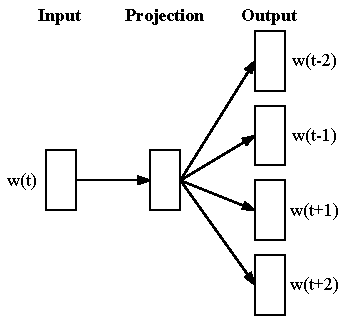
\includegraphics[width=\textwidth]{pic/skip_gram.pdf}
                \caption{Skip-gram.}
                \label{fig:first}
            \end{subfigure}
            \hfill
            \begin{subfigure}{0.4\textwidth}
                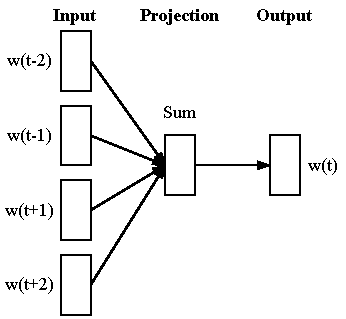
\includegraphics[width=\textwidth]{pic/cbow.pdf}
                \caption{CBOW.}
                \label{fig:second}
            \end{subfigure}
            \caption{Word embedding architectures. Adapted from \cite{mikolov2013efficient}.}
            \label{fig:word2vec_arquitecture}
        \end{figure}

        \begin{note}
            {Write your notes here}
        \end{note}
    \end{frame}

    \begin{frame}{Equations}
        \begin{equation}
            V = \frac{4}{3}\pi r^3
            \label{eq:vsphere}
        \end{equation}

        \begin{exampleblock}{Equation without numbers} 
            \begin{equation}
                J(\theta) = \mathbb{E}_{\pi_\theta}[G_t] = \sum_{s\in\mathcal{S}} d^\pi (s)V^\pi(s)=\sum_{s\in\mathcal{S}} d^\pi(s)\sum_{a\in\mathcal{A}}\pi_\theta(a|s)Q^\pi(s,a)
                \label{eq:train}
            \end{equation}
        \end{exampleblock}

        % \centering
        % Cosine similarity
        \begin{equation}
            cos(\theta) = \text{sim}(z_i, z_j) = \frac{z_i.z_j}{\|z_i\|\|z_j\|}
            \label{eq:cosine_similarity}
        \end{equation}
            
        \begin{note}
            {Write your notes here}
        \end{note}
    \end{frame}

    \begin{frame}{Equations multiline}
       \begin{exampleblock}{Equation with numbers}
            % Taken from Mathmode.tex
            \begin{multline}
                A=\lim_{n\rightarrow\infty}\Delta x\left(a^{2}+\left(a^{2}+2a\Delta x+\left(\Delta x\right)^{2}\right)\right.\label{eq:reset}\\
                +\left(a^{2}+2\cdot2a\Delta x+2^{2}\left(\Delta x\right)^{2}\right)\\
                +\left(a^{2}+2\cdot3a\Delta x+3^{2}\left(\Delta x\right)^{2}\right)\\
                +\ldots\\
                \left.+\left(a^{2}+2\cdot(n-1)a\Delta x+(n-1)^{2}\left(\Delta x\right)^{2}\right)\right)\\
                =\frac{1}{3}\left(b^{3}-a^{3}\right)
            \end{multline}
        \end{exampleblock}

        \begin{note}
            {Write your notes here}
        \end{note}
    \end{frame}

    \begin{frame}{Algorithm}
        \begin{algorithm}[H]
            \footnotesize
            \DontPrintSemicolon
            % \SetAlgoLined
            % \SetNoline
            
            \SetKwInOut{Input}{Input}
            \SetKwInOut{Output}{Output}
            
            \Input{An array $A$ of $n$ integers}
            \Output{Maximum element in the array}
            
            % \BlankLine
            % max $\leftarrow A[0]$\;
            % $X \gets x$\;
            %\For{$i \leftarrow 1$ \KwTo $n-1$}{
            %    \If{$A[i] >$ max}{
            %        max $\leftarrow A[i]$\ \Comment*[r]{This is a comment}
            %    }
            %}
            $y \gets 1$\;
            $X \gets x$\;
            $N \gets n$\;
            \While{$N \neq 0$}{
              \eIf{$N$ is even}{
                $X \gets X \times X$\;
                $N \gets \frac{N}{2}$ \Comment*[r]{This is a comment}
              }{\If{$N$ is odd}{
                  $y \gets y \times X$\;
                  $N \gets N - 1$\;
                }
              }
            }
            \Return max\;
            \caption{Find Maximum Element in an Array.}
            \label{tab:algorithm_new}
        \end{algorithm}
        
        \begin{note}
            {Write your notes here}
        \end{note}
    \end{frame}

\section{Section three}
    \begin{frame}{Tables}
        \begin{table}[ht!]
            \centering
            \caption{Definition.}
            \label{tab:table}
            \begin{tabular}{cllll}\toprule
                Eq. & Def. & A & B & C \\\midrule
                1 & 4.0 & 0 & 1 & 4.0 \\
                2 & 3.7 & 7 & 7 & 6.99 \\\bottomrule
            \end{tabular}
        \end{table}
        \normalsize Please check the definition of Equation~(\ref{eq:vsphere}) in Table~\ref{tab:table}.
        
        \begin{note}
            {Write your notes here}
        \end{note}
    \end{frame}
    
    \begin{frame}{Figures}   
        \begin{figure}[ht!]
            \centering
            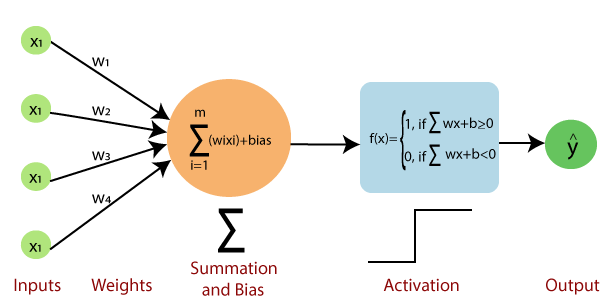
\includegraphics[width=0.86\linewidth]{pic/single-layer-perceptron-in-tensorflow2.png}
            \caption{Basic NN. \\
            From \url{https://www.javatpoint.com/single-layer-perceptron-in-tensorflow}.}
        \end{figure}

        \begin{note}
            {Write your notes here}
        \end{note}
    \end{frame}
   
    \begin{frame}{Video}
        \begin{figure}
            \centering
            % \includegraphics{}
            \animategraphics[width=1.0\textwidth, loop, autoplay]
            {5} % frame rate
            {pic/network_propagation/network-propagation_} % path to figures
            {0} % start index
            {71} % end index
            \caption{Image classification. From \url{https://www.3blue1brown.com/lessons/neural-networks}.}
            \label{fig:example_nn}
        \end{figure}

        \begin{note}
            {Write your notes here}
        \end{note}
    \end{frame}

\section*{References}
    \begin{frame}
        \begin{center}
            {\Huge\textit{Thank you for your attention!}}\\
            $\infty$ \\
            edwin.alvarez@pucp.edu.pe\\
            \url{https://github.com/win7}
        \end{center}
    \end{frame}
    
    %========================
    % bibliography
    %========================
    % \input{ref.bib}
    \begin{frame}[allowframebreaks]
        \bibliography{ref}
        % \bibliographystyle{unsrt}
        % \bibliographystyle{alpha}
        % If too many references, use this command to resize:
        \tiny\bibliographystyle{unsrt}
    \end{frame}

\end{document}